
\documentclass[12pt,a4paper]{article}
\usepackage{fullpage}
\usepackage[USenglish]{babel}
\usepackage{authblk}
\usepackage{hyperref}
\usepackage{graphicx}
\usepackage{listings}
\usepackage{xcolor}

\colorlet{punct}{red!60!black}
\definecolor{background}{HTML}{EEEEEE}
\definecolor{delim}{RGB}{20,105,176}
\colorlet{numb}{magenta!60!black}

\lstdefinelanguage{json}{
    basicstyle=\normalfont\ttfamily,
    numbers=left,
    numberstyle=\scriptsize,
    stepnumber=1,
    numbersep=8pt,
    showstringspaces=false,
    breaklines=true,
    frame=lines,
    backgroundcolor=\color{background},
    literate=
     *{0}{{{\color{numb}0}}}{1}
      {1}{{{\color{numb}1}}}{1}
      {2}{{{\color{numb}2}}}{1}
      {3}{{{\color{numb}3}}}{1}
      {4}{{{\color{numb}4}}}{1}
      {5}{{{\color{numb}5}}}{1}
      {6}{{{\color{numb}6}}}{1}
      {7}{{{\color{numb}7}}}{1}
      {8}{{{\color{numb}8}}}{1}
      {9}{{{\color{numb}9}}}{1}
      {:}{{{\color{punct}{:}}}}{1}
      {,}{{{\color{punct}{,}}}}{1}
      {\{}{{{\color{delim}{\{}}}}{1}
      {\}}{{{\color{delim}{\}}}}}{1}
      {[}{{{\color{delim}{[}}}}{1}
      {]}{{{\color{delim}{]}}}}{1},
}

\lstdefinelanguage{tableJson}{
    basicstyle=\small\ttfamily,
    showstringspaces=false,
    breaklines=true,
    aboveskip=0,
    belowskip=0,
    literate=
     *{0}{{{\color{numb}0}}}{1}
      {1}{{{\color{numb}1}}}{1}
      {2}{{{\color{numb}2}}}{1}
      {3}{{{\color{numb}3}}}{1}
      {4}{{{\color{numb}4}}}{1}
      {5}{{{\color{numb}5}}}{1}
      {6}{{{\color{numb}6}}}{1}
      {7}{{{\color{numb}7}}}{1}
      {8}{{{\color{numb}8}}}{1}
      {9}{{{\color{numb}9}}}{1}
      {:}{{{\color{punct}{:}}}}{1}
      {,}{{{\color{punct}{,}}}}{1}
      {\{}{{{\color{delim}{\{}}}}{1}
      {\}}{{{\color{delim}{\}}}}}{1}
      {[}{{{\color{delim}{[}}}}{1}
      {]}{{{\color{delim}{]}}}}{1},
}


\usepackage{todonotes}

% Remove section numbering
\setcounter{secnumdepth}{0}
% Remove paragraph indentation
\setlength{\parindent}{0cm}


\title{eBay Search Service \\[1ex] \large Preliminary Draft}
\author{Isabel Giang}
\author{Maxwell Wenger}
\affil{CSS490 Group Y4}

\date{January 26, 2021}


\begin{document}
\maketitle
\setcounter{tocdepth}{3}
\tableofcontents

% Problem:
% EBay Search has gotten quite slow.  We were able to gain some time by adding
% an index to the Master DB, but we are worried about long term scaling.  We
% need to settle on a design for a SearchServce that would be used to search
% for Auctions by Keyword and/or Category (breadcrumb)

% Deliverables:
% Create a design document that explains how you would solve the search
% problem.  This document will be read by the various engineers in the company
% for evaluation of your approach,so your design needs to be understandable to
% them based on the document.

\pagebreak
\section{Overview}
\subsection{Problem Statement}
In the last few months, eBay users have reported increasingly slow response
times from eBay's website when searching for auctions. Application log analysis
for the eBay Master Service has confirmed that our FindAuctions API for the
eBay Master service takes significantly longer to return a response when we
search for auctions using keywords. It also takes longer to search for a large
number of auctions.
\vspace{\baselineskip}
This is negatively impacting eBay's user experience for existing users and is
hindering the website's chances of being adopted by new users.

% State business problem
\vspace{\baselineskip}

Performing further analysis on the eBay Master service schema shows that the
FindAuctions API must scan the entire table to first find active auctions. Then
it must scan those active auctions to find auctions that have titles with the
keywords we are looking for.

\subsection{Temporary Solution}

As a bandaid solution to temporarily address this problem, we have added an 
AuctionStatus index to the Auction table of the eBay Master Service database.
This allows us to immediately access all active auctions instead of being forced 
to scan the entire Auction table to find active auctions before querying with keywords. 

\vspace{\baselineskip}
This speeds up the FindAuctions API enough to fix the poor user experience
temporarily, but this will not be enough as the company grows. The number of
records in the Auction table, and subsequently, the number of active auctions
will increase at an exponential rate.

\subsection{Next Steps}
To solve this more permanently, we want to create a separate search service
that will handle searching for auctions by keyword and/or category. 
We will call this new service the eBay Search Service. 

\vspace{\baselineskip}
This document will explain the following:

\begin{itemize}
    \item the API designs for each eBay Search Service API
    \item details needed for implementation and to assess if this solution is technically viable
    \item changes that must be made to the eBay Master Service to use the eBay Search Service
\end{itemize} 

\vspace{\baselineskip}
The search service will have its own database that can only be changed
by external users via its API. Whenever a new FindAuction API request is made, 
this service will perform the required business logic and databases accesses 
instead of the eBay Master service.

The eBay Search Service  will support searching in the following ways:

\begin{itemize}
    \item Searching for all auctions
    \item Searching for auctions based on auction status (closed, open, pending, cancelled)
    \item Searching for auctions based on keywords
    \item Searching for auctions based on category
    \item Searching for auctions based on keywords and category
\end{itemize}

Each search operation will only allow ``AND'' operations between search terms. 
For example, searching for auctions that have``red'' AND ``yellow'' in their titles.
\vspace{\baselineskip}

``OR'' operations must be done by forming a union of the results from multiple calls. 
For example, to get the results for auctions that have ``red'' OR ``yellow'' in their titles, 
you must combine the results of searching for auctions that have ``red" in their titles,
and the results of searching for auctions that have ``yellow'' in their titles.


\pagebreak
% Clarify what kinds of searching we are doing such as:
% - Allow searching for only active auctions 
% - this one -> Allow searching for any auction.
% - Allow a bidder to find all of their active auctions
% - Administrator looking for a specific set of auctions that have expired
% - Etc

% Need Database Schema
 
\section{eBay Search Service API Specification}

\subsection{API List}
\begin{center}
    \begin{tabular}{| l | l |}
        \hline
        \textbf{API Name} & \textbf{Description} \\
        \hline
            saveSearchableAuction & Updates or creates a searchable auction \\ 
        \hline
            removeSearchableAuction & Removes an auction. \\
        \hline
            findAuctions & Finds auctions based on the given keywords and/or category. \\
        \hline
    \end{tabular}
\end{center}

\subsection{Schemas}

\subsubsection{SearchDB}
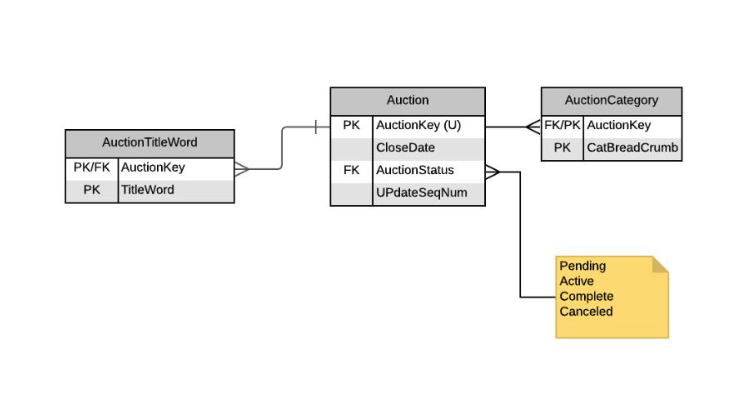
\includegraphics[scale=0.5]{images/search-schema.png}
\subsubsection{MasterDB}
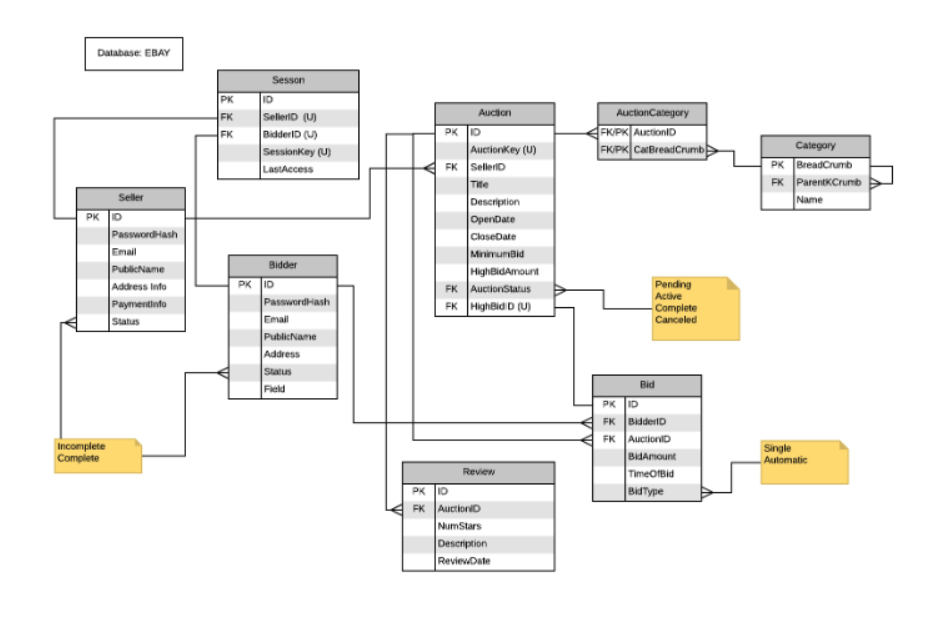
\includegraphics[scale=0.35]{images/master-schema.png}
\pagebreak
\subsection{API Descriptions}

\subsubsection{saveSearchableAuction}
\label{ref:csa}
Updates an existing auction or creates one if no auction with the auction key
exists.

\paragraph{Input}

\begin{itemize}
    \item \textbf{auctionKey} - Public key that uniquely identifies an auction from the eBay Master Service.
    \item \textbf{title} - Title of the auction 
    \item \textbf{closeDate} - Closing date of the auction (ISO-8601 timestamp)
    \item \textbf{category} - Category breadcrumb
    \item \textbf{status} - Status of the auction (closed, open, pending, cancelled)
    \item \textbf{seqNum} - Sequence number of the auctions table. Each time
        there is an update, it is incremented by one. Requests made with
        smaller sequence numbers than the one in the database are ignored.
\end{itemize}
\begin{lstlisting}[language=json,numbers=none]
{
    "auctionKey": <string>,
    "title": <string>,
    "closeDate": <string>,
    "categories": [ <string>, ...],
    "status": <string>,
    "seqNum": <int>
}
\end{lstlisting}

\paragraph{Output}
\begin{center}
    \begin{tabular}{| p{5cm} | l |}
        \hline
        \textbf{Scenario} & \textbf{Response} \\
        \hline
        Successfully saved an auction & 
        \begin{lstlisting}[language=tableJson,firstnumber=1]
{
    "success": true,
    "seqNum": <int> // current seq num in
                    // the database.
}

        \end{lstlisting} \\ 
        \hline
    \end{tabular}
\end{center}



\pagebreak
\subsubsection{findAuctions}

findAuctions will return a number of results based on the user's query. The
parameters search by ``anding'' the results together (e.g. if you ask for a
keyword ``red'', ``LG'' with the category ``ELE:PHO'' signifying phones in
electronics, red LG phones will be returned, but not red Nokia phones, or red
LG refrigerators). To perform searches that ``or'' search terms, multiple
searches must be made. lastAuctionKey and numResults are to be used for
pagination. findAuctions will return numResults number of entries ordered from
oldest to newest, starting from the lastAuctionKey. If no lastAuctionKey is
provided, findAuctions will return numResults number of results starting from
the first result.

\paragraph{Input} 

\begin{itemize}
    \item \textbf{keywords} - Keywords that auction results will be matched to
    \item \textbf{category} - Category breadcrumb
    \item \textbf{status} - Status of the auction (closed, open, pending, cancelled)
    \item \textbf{lastAuctionKey} - The last auction key will be last auction
        not included in the results that are numResults long. If given, results
        will be returned starting from this page.
    \item \textbf{numResults} - Number of auctions returned per page
\end{itemize}

\begin{lstlisting}[language=json,numbers=none]
{
    "keywords": [ <string>, ...], // optional
    "status": <string>, // optional
    "categories": [<string>, ...], // optional
    "lastAuctionKey": <number>, // optional
    "numResults": <number>
}
\end{lstlisting}

\paragraph{Output}
\begin{center}
    \begin{tabular}{| p{7cm} | l |}
        \hline
        \textbf{scenario} & \textbf{response} \\
        \hline
        Successfully search with found results. &
        \begin{lstlisting}[language=tablejson,firstnumber=1]
{
    "success": true,
    "results": [ 
        auctionKey: <string>,
        ...
    ],
    "pageIndex": <int>
}
        \end{lstlisting} \\ 
        \hline
 \hline
        Successfully search with no results. &
        \begin{lstlisting}[language=tablejson,firstnumber=1]
{
    "success": true,
    "results": [ ]
}
         \end{lstlisting} \\ 
        % \hline
         %    todo: make error states & yeah! what he said! \\
         \hline
    \end{tabular}
\end{center}

\pagebreak
\section{eBay Search Service Internals}
% Describe what internal processes you do based on APIs.
% I.E. What happens to DB when xyz is called.
\subsection{saveSearchableAuction}
saveSearchableAuction will update fields, keywords, and categories of an
existing auction in the search table.

New keywords will be generated if a new title is provided. The new keywords
will be added to the database, and keywords associated with they auction key
but were not again generated from the updated title will be removed from the
database. The fields will be based on the auction key, therefore the auction
key may not be updated. Any optional fields not included in the message to the
service will not be changed. To remove a title, an empty string must be
provided (``''). If an empty string is provided, all keywords will be deleted
as before, but no new ones will be generated.

\subsection{removeSearchableAuction}
Remove searchable auction does simply that. It will delete the keywords and
category entries from each table matching the auction key that was requested to
be deleted. In general, its not good practice to delete things out of the
database, but in the case, its okay because this the search database is treated
more like a cache than a datastore. The original data will still exist in the
main database.

\subsection{findAuctions}
Find auctions builds a query based on the provided information. It generates
this query as an ``and'' operation, so results passed back are only those that
fit all the criteria you passed to findAuction. It handles pagination by having
the user keep track of the last auction it saw, and request a certain number
after that. So from our ordered query, we will pull numResults of results back,
starting from one after the last auction key. If the last auction key was
deleted/does not exist at the time of the call, it will return numResults
number of results starting from the first value again. This helps get around
the issue of missed auctions that were added during the search session.

\pagebreak
\section{Changes to eBay Master Service}

\subsection{MasterDB Schema Changes}
The \texttt{SeqNum} field has been added to the \texttt{Auction} table to count and
uniquely identify the order of new transactions and the number of new auctions 
that have been added to the table. 


\subsection{eBay Master API Definition Changes}

\subsubsection{createAuction}
After creating a new entry in the MasterDB's Auction table as part of a transaction, 
the \texttt{createAuction} API must call the eBay Search Service's 
\texttt{saveSearchableAuction} API to trigger a transaction to create 
a new auction in the SearchDB, sending a \texttt{SeqNum}.
\texttt{SeqNum} begins at 0, and increments by 1 each time an auction is added.

\vspace{\baselineskip}
The eBay Master Service will then receive a response from the eBay Search Service. 
If the response does not return \texttt{"success":"true"}, with a \texttt{seqNum}
larger than or equal to the \texttt{seqNum} originally sent by the ebay Master Service, 
the eBay Master Service will fail the transaction, roll back the creation of the new Auction record, 
and send an response back to the user of the \texttt{createAuction} API 
indicating an error has occurred.


\vspace{\baselineskip}
Aside from updating SeqNum each time a new auction is created, the 
impact on the MasterDB from performing \texttt{createAuction} is the same as 
documented in the eBay Master Service API specification.

% For any changes to the ebay master service, we need to provide:
% - Description of schema changes (not a full schema drawing)
% - Description of behavioral changes
%   - Describe new control  flow
%   - Describe transactional events
%   - Describe what happens on timeout from the search service.
% - Any additional API calls that are needed to be added to master service

\subsubsection{updateAuction}

After successfully updating an auction in the MasterDB Auction table as part of a transaction, 
 \texttt{updateAuction} will call \texttt{saveSearchableAuction} and increment \texttt{SeqNum} 
 in the MasterDB Auction table by one.

 \vspace{\baselineskip} 

The eBay Master Service will then receive a response from the eBay Search Service.
If the response does not return \texttt{"success":"true"}, with a \texttt{seqNum}
larger than or equal to the \texttt{seqNum} originally sent by the ebay Master Service, 
the eBay Master Service will fail the transaction, roll back the creation of the new Auction record, 
and send an response back to the user of the \texttt{updateAuction} API 
indicating an error has occurred.

\vspace{\baselineskip} 
Aside from updating SeqNum each time an auction is updated, the 
impact on the MasterDB from performing \texttt{createAuction} is the same as 
documented in the eBay Master Service API specification.

\subsubsection{findOpenAuctions}
This service in the master DB now simply calls the findAuctions service from
the search service, passing through the keywords and category it was passed,
but only looking for auctions with a status of open.

\pagebreak
\section{Logging}

This section describes a suggested format for this service's application logs.

\begin{lstlisting}[boxpos=t,language=json,firstnumber=1]
{
    "start": <string>,
    "duration": <string>,
    "api": <string>,
    "params":
        {
            "original": {
                "auctionkey": <string>,
                "title": <string>,
                "closeDate": <string>,
                "status": <string>, 
                "category": [<string>, ...],
                "seqNum": <int> 
            }, 
            "updated": {
                "auctionkey": <string>,
                "title": <string>,
                "closeDate": <string>,
                "status": <string>,
                "category": [<string>, ...],
                "seqNum": <int> 
            }
        }
}           
\end{lstlisting}

\begin{itemize}
    \item \textbf{start} The time the service first receives the call.
    \item \textbf{duration} The amount of time it takes from when the service
        receives the call to when the service responds.
    \item \textbf{api} The name of the API that is called.
    \item \textbf{params} The original and updated data that the API changed.
        Optional data that was not changed is not included in either the
        updated or original logs.
\end{itemize}


\end{document}
